\begin{table*}[hbtp]
    \centering
    \begin{tabular}{cc|ccc|ccc}
        %\cline{3-8}
        \multicolumn{2}{c}{} & \multicolumn{3}{|c|}{Analytical} & \multicolumn{3}{c}{Numerical} \\
        \hline
         $N_{part}$ & $N_{dim}$ & $E \ [\sigma^2_E]$ & $T_{run}$ & $acceptance$ & $E \ [\sigma^2_E]$ & $T_{run}$ & $acceptance$ \\
         \hline
         $1$ & $1$ & $0 \ [0]$ & $0$ & $0$  & $0 \ [0]$ & $0$ & $0$ \\
         $1$ & $2$ & $0 \ [0]$ & $0$ & $0$  & $0 \ [0]$ & $0$ & $0$ \\
         $1$ & $3$ & $0 \ [0]$ & $0$ & $0$  & $0 \ [0]$ & $0$ & $0$ \\
         \hline
         $10$ & $1$ & $0 \ [0]$ & $0$ & $0$  & $0 \ [0]$ & $0$ & $0$ \\
         $10$ & $2$ & $0 \ [0]$ & $0$ & $0$  & $0 \ [0]$ & $0$ & $0$ \\
         $10$ & $3$ & $0 \ [0]$ & $0$ & $0$  & $0 \ [0]$ & $0$ & $0$ \\
         \hline
         $50$ & $1$ & $0 \ [0]$ & $0$ & $0$  & $0 \ [0]$ & $0$ & $0$ \\
         $50$ & $2$ & $0 \ [0]$ & $0$ & $0$  & $0 \ [0]$ & $0$ & $0$ \\
         $50$ & $3$ & $0 \ [0]$ & $0$ & $0$  & $0 \ [0]$ & $0$ & $0$ \\
         \hline
         $100$ & $1$ & $0 \ [0]$ & $0$ & $0$  & $0 \ [0]$ & $0$ & $0$ \\
         $100$ & $2$ & $0 \ [0]$ & $0$ & $0$  & $0 \ [0]$ & $0$ & $0$ \\
         $100$ & $3$ & $0 \ [0]$ & $0$ & $0$  & $0 \ [0]$ & $0$ & $0$ \\
         \hline
    \end{tabular}
    \caption{\bfseries Non-interacting Metropolis analysis}{The table reports the results of the simulations of the non-interacting case using a simple gaussian trial wavefunction and a brute force Metropolis sampling method. The variational parameter was kept fixed at the value $\alpha^{best}=0.5$. The Metropolis step-size was set to $h=0.01$.}
    \label{tab:tab_x_metropolis}
    \vspace{15pt}
    \centering
    \begin{tabular}{cc|ccc|ccc}
        %\cline{3-8}
        \multicolumn{2}{c}{} & \multicolumn{3}{|c|}{Analytical} & \multicolumn{3}{c}{Numerical} \\
        \hline
         $N_{part}$ & $N_{dim}$ & $E \ [\sigma^2_E]$ & $T_{run}$ & $acceptance$ & $E \ [\sigma^2_E]$ & $T_{run}$ & $acceptance$ \\
         \hline
         $1$ & $1$ & $0 \ [0]$ & $0$ & $0$  & $0 \ [0]$ & $0$ & $0$ \\
         $1$ & $2$ & $0 \ [0]$ & $0$ & $0$  & $0 \ [0]$ & $0$ & $0$ \\
         $1$ & $3$ & $0 \ [0]$ & $0$ & $0$  & $0 \ [0]$ & $0$ & $0$ \\
         \hline
         $10$ & $1$ & $0 \ [0]$ & $0$ & $0$  & $0 \ [0]$ & $0$ & $0$ \\
         $10$ & $2$ & $0 \ [0]$ & $0$ & $0$  & $0 \ [0]$ & $0$ & $0$ \\
         $10$ & $3$ & $0 \ [0]$ & $0$ & $0$  & $0 \ [0]$ & $0$ & $0$ \\
         \hline
         $50$ & $1$ & $0 \ [0]$ & $0$ & $0$  & $0 \ [0]$ & $0$ & $0$ \\
         $50$ & $2$ & $0 \ [0]$ & $0$ & $0$  & $0 \ [0]$ & $0$ & $0$ \\
         $50$ & $3$ & $0 \ [0]$ & $0$ & $0$  & $0 \ [0]$ & $0$ & $0$ \\
         \hline
         $100$ & $1$ & $0 \ [0]$ & $0$ & $0$  & $0 \ [0]$ & $0$ & $0$ \\
         $100$ & $2$ & $0 \ [0]$ & $0$ & $0$  & $0 \ [0]$ & $0$ & $0$ \\
         $100$ & $3$ & $0 \ [0]$ & $0$ & $0$  & $0 \ [0]$ & $0$ & $0$ \\
         \hline
    \end{tabular}
    \caption{\bfseries Non-interacting Importance Sampling analysis}{The table reports the results of the simulations of the non-interacting case using a simple gaussian trial wavefunction and the Importance Sampling method. The variational parameter was kept fixed at the value $\alpha^{best}=0.5$. The time step-size was set to $\delta t = 0.01$.}
    \label{tab:tab_x_importance}
    
    \vspace{15pt}
    \centering
    \begin{tabular}{c|ccc|ccc}
        %\cline{3-8}
         & \multicolumn{3}{c|}{Metropolis} & \multicolumn{3}{c}{Importance Sampling} \\
        \hline
         $\alpha$ & $E$ & $\sigma^2_E/N$ & $\sigma^2_B$ & $E$ & $\sigma^2_E/N$ & $\sigma^2_B$ \\
         \hline
         $0.3$ & $0$ & $0$ & $0$ & $0$  & $0$ & $0$ \\
         $0.4$ & $0$ & $0$ & $0$ & $0$  & $0$ & $0$ \\
         $0.5$ & $0$ & $0$ & $0$ & $0$  & $0$ & $0$ \\
         $0.6$ & $0$ & $0$ & $0$ & $0$  & $0$ & $0$ \\
         $0.7$ & $0$ & $0$ & $0$ & $0$  & $0$ & $0$ \\
         $0.8$ & $0$ & $0$ & $0$ & $0$  & $0$ & $0$ \\
         \hline
    \end{tabular}
    \caption{The table reports the results of the simulations for different values of the variational parameter $\alpha$. For both the Metropolis case and the Importance Sampling case we used 10 particles in 3 dimensions and $2^{21}$ steps. The chosen step-size for the Metropolis algorithm was $h/a_{ho}=0.01$ and the time step-size for the Importance Sampling was $\delta t = 0.01$.}
    \label{tab:varying_alpha_noninteracting}
\end{table*}

The analysis of the results produced by our algorithm passed through a series of intermediate and progressive steps continuously checking the results obtained via the simulation with the analytical formulas, fortunately available for the non-interacting case.
\subsection{NON-INTERACTING SYMMETRICAL CASE}
At first we chose a spherical potential trap with a simple gaussian trial wavefunction (see Eq.\,\ref{potential} and Eq.\,\ref{wavefunctions}). The algorithm chosen to obtain a numerical estimation of the ground state energy of the system was the so called Brute-Force Metropolis algorithm, previously introduced. We performed different simulations varying different parameters of the system. Before each simulation the system was submitted to $10^5$ thermalization steps. ( \textit{Commento sul fatto che questo numero è stato tenuto fisso per ogni simulazione})
Table \ref{tab:tab_x_metropolis} reports the results of the analysis of the system's dependence on the number of particles and dimension. The value of $\alpha$ was kept fixed at $\alpha^{best} = 0.5$. Instead, figure \ref{fig:varying_alpha_noninteract_metropolis}, shows the value of the ground state energy of the system as a function of the parameter $\alpha$ for a particular configuration of the simulation settings, that is 10 particles, 3 dimensions, $2^{21}$ steps and Metropolis step-size $h = 0.01$. \\ One can immediately notice that the function is convex, which guarantees the existence of one unique minimum point: this is a fundamental fact for what concerns the gradient descent method, as we discussed before. Some selected results for different $\alpha$ values are reported also in table \ref{tab:varying_alpha_noninteracting}. This table contains also a comparison between the variance of the energies $\sigma^2_E$ calculated as $\sigma^2_E = \left\langle E_L^2 \right\rangle - \left\langle E_L \right\rangle^2$ and the variance calculated via the blocking method as explained in section \ref{variance}.
\begin{figure}[H]
    \centering
    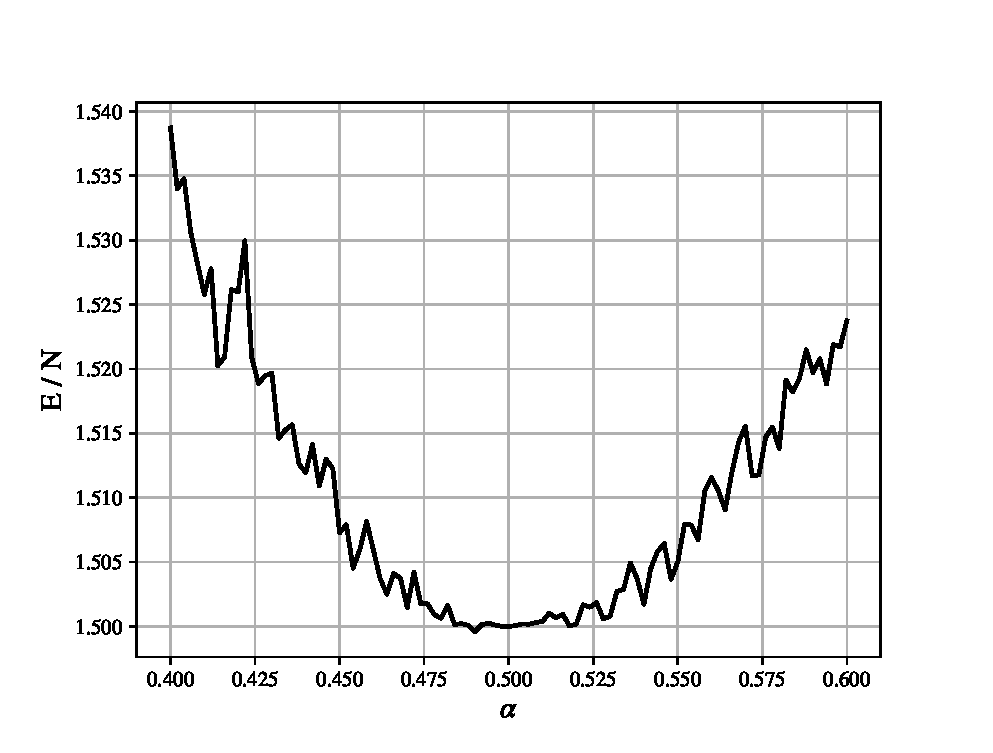
\includegraphics[scale=0.5]{images/varying_alpha_noninteract.eps}
    \caption{Grafico molto di prova Metropolis}
    \label{fig:varying_alpha_noninteract_metropolis}
\end{figure}


The immediate improvement of this simple model was the inclusion of the importance sampling. This allowed us to bias the random walk in the configuration space according to the probability distribution leading to higher number of accepted steps in the Monte Carlo with the same parameters. Note that since the particles are now biased to move towards region of higher probability (e.g. the origin), more Monte Carlo cycles are required to find the particles far enough from the origin to obtain a significant result. As for the Brute Force Metropolis, results for fixed $\alpha$ are reported in table \ref{tab:tab_x_importance}, while the estimated energy as a function of $\alpha$ is reported in figure \ref{fig:varying_alpha_noninteract_importance} with some selected results in table \ref{tab:varying_alpha_noninteracting}. \\
\begin{figure}[H]
    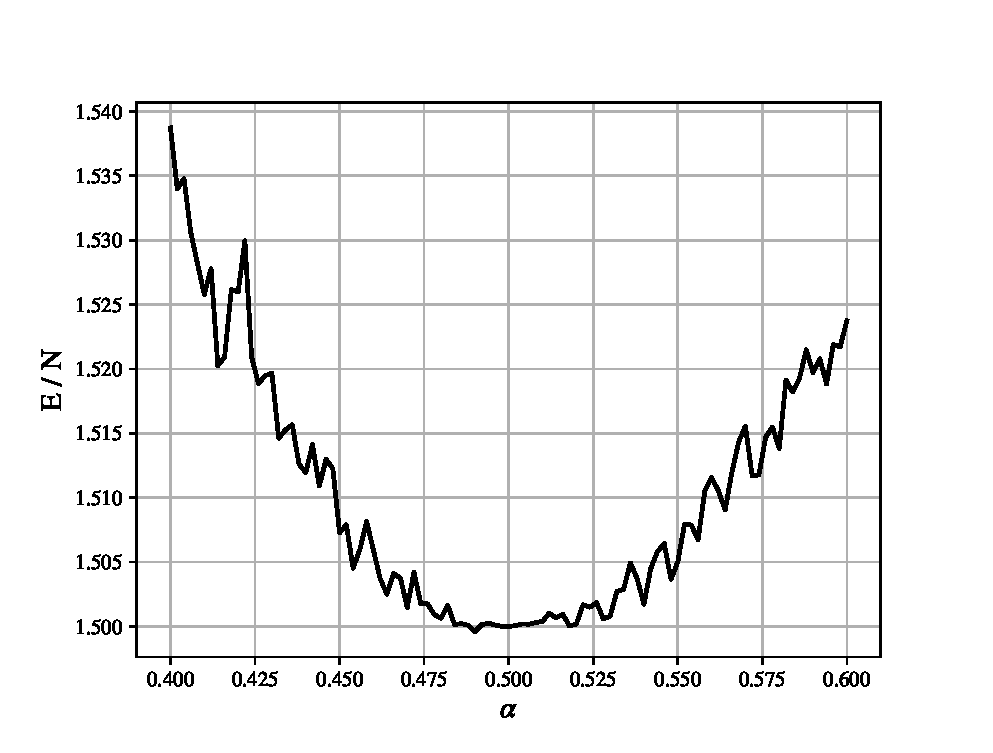
\includegraphics[scale=0.5]{images/varying_alpha_noninteract.eps}
    \caption{Grafico molto di prova Importance}
    \label{fig:varying_alpha_noninteract_importance}
\end{figure}
Even if simple and primitive, this model allowed us to test many of the fundamental parts of the project and made us understand how to fine-tune some parameters involved in the problem. For example we analysed the effects of the time step-length $\delta t$ in the importance sampling case (see figure \ref{fig:dt_importance_sampling}) concluding that a good choice for the parameter could be $\delta t = 0.01$. \\
The last test on this system was the numerical approach, in which we calculated the local energy numerically starting from the wavefunction expression. Results of the simulations are reported next to the analytical corresponding cases in tables \ref{tab:tab_x_importance} and \ref{tab:tab_x_metropolis}. One can notice a significant increase in the simulation time with the numerical approach, hence leaving the only purpose of this method to perform fast tests and qualitative studies.
\begin{figure}[H]
    \centering
    \includegraphics[scale=0.45]{images/time_steplength.png}
    \caption{I will do a nicer plot, it is just to keep the flow}
    \label{fig:dt_importance_sampling}
\end{figure}


\begin{table*}[h]
\centering
 \begin{tabular}{c|c|c|c|}
         & \multicolumn{3}{c|}{Importance} \\
        \hline
         Starting $\alpha$ & $\gamma$ & $N_{step}$ & Final $\alpha$ \\
       \hline
          & $0$ & $0$ & $0$ \\
         $0.4$ & $0$ & $0$ & $0$ \\
          & $0$ & $0$ & $0$ \\
         \hline
          & $0$ & $0$ & $0$ \\
         $0.6$ & $0$ & $0$ & $0$ \\
          & $0$ & $0$ & $0$ \\
         \hline
    \end{tabular}
    \caption{The table reports the results of the gradient descent method starting from $\alpha=0.4$ and $\alpha=0.6$. The simulations of the non-interacting case using a simple gaussian trial wavefunction and the Importance Sampling method. We used 10 particles in 3 dimensions and $10^5$ Monte Carlo steps. We used $10^5$ steps to thermalize the system. The timestep-size was set to $\delta t= 0.01$  }
\end{table*}

\subsubsection*{Interacting case}
We then moved on to the interacting and asymmetrical case with trial wavefunction given by \ref{wavefunctions} and hamiltonian given by \ref{hamiltonian}. At first we compared results with those obtained from the symmetrical case: this could be done by setting $\beta=1$, $w_z = w_{ho}$ and the s-wave scattering length $a$ to 0. After this check we set the parameters values $\omega_z/\omega_{ho} = \sqrt{8} = \beta$ and $a/a_{ho} = 0.0043$ and ran the simulations for $N=10,50,100$ particles varying $\alpha$. As an example, results for 10 particles, are reported in figure \ref{fig_asymm_symm_comparions} and compared to the non-interacting symmetrical case. In addition figure \ref{fig:E_over_N} reports a comparison between the energies per particle as a function of the variational parameter $\alpha$ obtained for the three different values of $N$. \\
Again we found a convex function with unique minimum: this allowed us to perform a gradient descent to obtain the value $\alpha^{best}$. Though, in this case, the problem was less trivial since the optimal value of the variational parameter depends also on the chosen number of particles and on the starting value of $\alpha$. Our analysis is resumed in tables \ref{tab:best_alpha_N_fixed} and \ref{tab:optimal_alpha}.

\begin{table}[H]
    \centering
    \begin{tabular}{c|cc|cc}
            & \multicolumn{2}{c}{$\gamma_1=10^{-2}$} & \multicolumn{2}{|c|}{$\gamma_2=10^{-3}$} \vspace{1pt}\\
            \hline
            $\alpha^{start}$ & $\alpha^{best}$ & $N_{steps}$ & $\alpha^{best}$ & $N_{steps}$\\
            \hline
            $0$ & $0$ & $0$ & $0$ & $0$ \\
            $0$ & $0$ & $0$ & $0$ & $0$ \\
            $0$ & $0$ & $0$ & $0$ & $0$ \\
            \hline
        \end{tabular}
    \caption{Convergence analysis of the gradient descent method for fixed number of particles ($N=10$), importance sampling time step-size $\delta t = 0.01$, $2^{21}$ Monte Carlo steps and tolerance $10^{-8}$????}
    \label{tab:best_alpha_N_fixed}
\end{table}

\begin{table}[H]
    \centering
    \begin{tabular}{c|c|c|c|c}
            $N$ & $\alpha^{best}$ & $E$ & $\sigma^2_B$ & acceptance \\
            \hline
            10 & $0$ & $0$ & $0$ & $0$ \\
            50 & $0$ & $0$ & $0$ & $0$ \\
            100 & $0$ & $0$ & $0$ & $0$ \\
            \hline
        \end{tabular}
    \caption{Caption}
    \label{tab:optimal_alpha}
\end{table}